\documentclass{standalone}
\usepackage{tikz}
\usetikzlibrary{positioning, calc}

\begin{document}
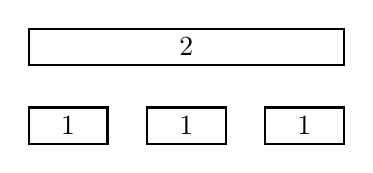
\begin{tikzpicture}[c/.style = {draw, thick, minimum width = #1}]
  \node (c2) [c = 4cm] {$2$};
  \node (c1) [c = 1cm, below = 1.0cm of c2.west, anchor = west] {$1$};
  \node (c11) [c = 1cm, below = 1.0cm of c2.center, anchor = center] {$1$};
  \node (c111) [c = 1cm, below = 1.0cm of c2.east, anchor = east] {$1$};
\end{tikzpicture}
\end{document}
